


\tikzset{every picture/.style={line width=0.75pt}} %set default line width to 0.75pt        

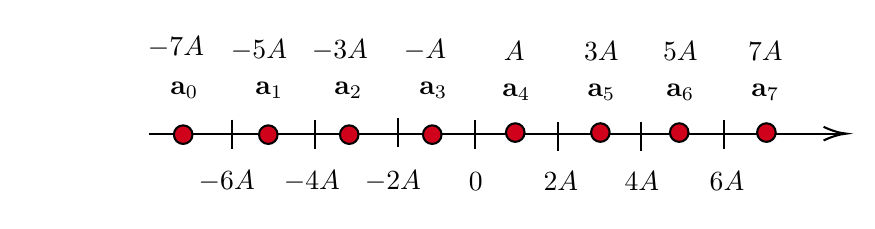
\begin{tikzpicture}[x=0.75pt,y=0.75pt,yscale=-1,xscale=1]
%uncomment if require: \path (0,300); %set diagram left start at 0, and has height of 300

%Straight Lines [id:da0785677110363594] 
\draw    (173.96,114) -- (507.96,114) ;
\draw [shift={(509.96,114)}, rotate = 180] [color={rgb, 255:red, 0; green, 0; blue, 0 }  ][line width=0.75]    (10.93,-3.29) .. controls (6.95,-1.4) and (3.31,-0.3) .. (0,0) .. controls (3.31,0.3) and (6.95,1.4) .. (10.93,3.29)   ;

%Shape: Circle [id:dp8429373004294252] 
\draw  [fill={rgb, 255:red, 208; green, 2; blue, 27 }  ,fill opacity=1 ] (306,114.48) .. controls (306,112.01) and (308.01,110) .. (310.48,110) .. controls (312.96,110) and (314.96,112.01) .. (314.96,114.48) .. controls (314.96,116.96) and (312.96,118.96) .. (310.48,118.96) .. controls (308.01,118.96) and (306,116.96) .. (306,114.48) -- cycle ;
%Straight Lines [id:da9917337286598218] 
\draw    (330.96,107.29) -- (330.96,121.29) ;


%Shape: Circle [id:dp31317929420387847] 
\draw  [fill={rgb, 255:red, 208; green, 2; blue, 27 }  ,fill opacity=1 ] (266,114.48) .. controls (266,112.01) and (268.01,110) .. (270.48,110) .. controls (272.96,110) and (274.96,112.01) .. (274.96,114.48) .. controls (274.96,116.96) and (272.96,118.96) .. (270.48,118.96) .. controls (268.01,118.96) and (266,116.96) .. (266,114.48) -- cycle ;
%Shape: Circle [id:dp8703696009425539] 
\draw  [fill={rgb, 255:red, 208; green, 2; blue, 27 }  ,fill opacity=1 ] (227,114.48) .. controls (227,112.01) and (229.01,110) .. (231.48,110) .. controls (233.96,110) and (235.96,112.01) .. (235.96,114.48) .. controls (235.96,116.96) and (233.96,118.96) .. (231.48,118.96) .. controls (229.01,118.96) and (227,116.96) .. (227,114.48) -- cycle ;
%Shape: Circle [id:dp48312291319442124] 
\draw  [fill={rgb, 255:red, 208; green, 2; blue, 27 }  ,fill opacity=1 ] (186,114.48) .. controls (186,112.01) and (188.01,110) .. (190.48,110) .. controls (192.96,110) and (194.96,112.01) .. (194.96,114.48) .. controls (194.96,116.96) and (192.96,118.96) .. (190.48,118.96) .. controls (188.01,118.96) and (186,116.96) .. (186,114.48) -- cycle ;
%Shape: Circle [id:dp32010417887626774] 
\draw  [fill={rgb, 255:red, 208; green, 2; blue, 27 }  ,fill opacity=1 ] (467,113.48) .. controls (467,111.01) and (469.01,109) .. (471.48,109) .. controls (473.96,109) and (475.96,111.01) .. (475.96,113.48) .. controls (475.96,115.96) and (473.96,117.96) .. (471.48,117.96) .. controls (469.01,117.96) and (467,115.96) .. (467,113.48) -- cycle ;
%Shape: Circle [id:dp665622950437736] 
\draw  [fill={rgb, 255:red, 208; green, 2; blue, 27 }  ,fill opacity=1 ] (425,113.48) .. controls (425,111.01) and (427.01,109) .. (429.48,109) .. controls (431.96,109) and (433.96,111.01) .. (433.96,113.48) .. controls (433.96,115.96) and (431.96,117.96) .. (429.48,117.96) .. controls (427.01,117.96) and (425,115.96) .. (425,113.48) -- cycle ;
%Shape: Circle [id:dp5860873971209044] 
\draw  [fill={rgb, 255:red, 208; green, 2; blue, 27 }  ,fill opacity=1 ] (387,113.48) .. controls (387,111.01) and (389.01,109) .. (391.48,109) .. controls (393.96,109) and (395.96,111.01) .. (395.96,113.48) .. controls (395.96,115.96) and (393.96,117.96) .. (391.48,117.96) .. controls (389.01,117.96) and (387,115.96) .. (387,113.48) -- cycle ;
%Shape: Circle [id:dp20437801267978872] 
\draw  [fill={rgb, 255:red, 208; green, 2; blue, 27 }  ,fill opacity=1 ] (346,113.48) .. controls (346,111.01) and (348.01,109) .. (350.48,109) .. controls (352.96,109) and (354.96,111.01) .. (354.96,113.48) .. controls (354.96,115.96) and (352.96,117.96) .. (350.48,117.96) .. controls (348.01,117.96) and (346,115.96) .. (346,113.48) -- cycle ;
%Straight Lines [id:da51291390000777] 
\draw    (370.96,108.29) -- (370.96,122.29) ;


%Straight Lines [id:da2811648906641422] 
\draw    (410.96,108.29) -- (410.96,122.29) ;


%Straight Lines [id:da4403380546942397] 
\draw    (450.96,107.29) -- (450.96,121.29) ;


%Straight Lines [id:da9495765085027235] 
\draw    (213.96,107.29) -- (213.96,121.29) ;


%Straight Lines [id:da24674873474006298] 
\draw    (253.96,107.29) -- (253.96,121.29) ;


%Straight Lines [id:da44203695518931974] 
\draw    (293.96,106.29) -- (293.96,120.29) ;



% Text Node
\draw (331.48,136.96) node   {$0$};
% Text Node
\draw (120,142) node   {$$};
% Text Node
\draw (191,93) node   {$\mathbf{a}_{0}$};
% Text Node
\draw (232,93) node   {$\mathbf{a}_{1}$};
% Text Node
\draw (270,93) node   {$\mathbf{a}_{2}$};
% Text Node
\draw (311,93) node   {$\mathbf{a}_{3}$};
% Text Node
\draw (351,94) node   {$\mathbf{a}_{4}$};
% Text Node
\draw (392,94) node   {$\mathbf{a}_{5}$};
% Text Node
\draw (430,94) node   {$\mathbf{a}_{6}$};
% Text Node
\draw (471,94) node   {$\mathbf{a}_{7}$};
% Text Node
\draw (187,72.5) node   {$-7A$};
% Text Node
\draw (227,74) node   {$-5A$};
% Text Node
\draw (266,74) node   {$-3A$};
% Text Node
\draw (307,74) node   {$-A$};
% Text Node
\draw (350,74) node   {$A$};
% Text Node
\draw (392,74) node   {$3A$};
% Text Node
\draw (430,74) node   {$5A$};
% Text Node
\draw (471,74) node   {$7A$};
% Text Node
\draw (372.48,136.96) node   {$2A$};
% Text Node
\draw (411.48,136.96) node   {$4A$};
% Text Node
\draw (452.48,136.96) node   {$6A$};
% Text Node
\draw (211.48,136.96) node   {$-6A$};
% Text Node
\draw (252.48,136.96) node   {$-4A$};
% Text Node
\draw (291.48,136.96) node   {$-2A$};


\end{tikzpicture}

